\documentclass[a4paper]{article}

%Packages
\usepackage[swedish]{babel}
\usepackage[T1]{fontenc}
\usepackage[utf8]{inputenc}
\usepackage{graphicx}
\usepackage{float}

\newcommand\namn{Larmsystem}

\restylefloat{table}

\begin{document}

%
% Front page
%

\thispagestyle{empty}

\begin{center}
    \parskip=14pt%
    \vspace*{3\parskip}%

    {\LARGE Projektplan DAT290}

    {\large \namn, grupp 11

    Titus Blosse, Viktor Frideen, Nazif Kadiroglu, Markus Moen, Lukas Schiavone, Fredrik Österström

    \today}

    \rule{7cm}{0.4pt}\\
\end{center}
\newpage

%
% ToC, Table of Contents
%

\thispagestyle{empty}

\tableofcontents
\newpage

%
% Projektplan
%

\pagenumbering{arabic}

% Kategorisera här, typ introduktion, teknisk beskrivnin...
\section{Syfte}

75.250 inbrott anmäldes i Sverige år 2019. En minskning med 14\% från året innan \cite{brastold}. Larmsystemet minskar risken för ett inbrott och möjliggör ytterligare minskning i Sverige. % Skriv resten av världen här

%Därför har vi valt att utveckla ett larm som enkelt kan installeras i alla typer av bostäder och som ger ett grundligt skydd mot oönskat intrång. Vi eftersträvar att i den slutgiltiga produkten kunna erbjuda en rad olika larmkomponenter som enkelt kan anslutas till en larmcentral och konfigureras för att passa kundens specifika sitution.
%I Sverige anmäldes 75250 inbrottsstölder år 2019 vilket är en minskning med 14\%\ från året innan \cite{brastold}. Detta är en trend som vi gärna ser hålla i sig. Därför har vi valt att utveckla ett larm som kan installeras i många typer av bostäder och som ger ett grundligt skydd mot oönskat intrång.

%Detta syfte kanske är lite för bakgrundigt?
% År borde inte vara i fokus, kanske börja med 75250 eller inbrottsstölder som meningen handlar om
% !Enkelt

\section{Mål}

%Vi strävar efter att utveckla ett system som ska ge användaren bättre kontroll och övervakningsmöjligheter över sina tillhörigheter.

Slutgiltiga produkten ska erbjuda ett flertal larmkomponenter som kan anslutas till en larmcentral och konfigureras för att passa kundens specifika sitution. Systemet ska vara dokumenterat och fackmannamässigt utfört med förutsättningar för expansion.

Grunden i systemet kommer vara en centralenhet till vilken användaren kan ansluta periferienheter. Huvudsakligen kommer två periferienheter att utvecklas, ett dörrlarm och ett rörelselarm. I mån av tid kommer också systemets funktionalitet utökas. Ett testläge för systemet, möjlighet att konfigurera rörelselarmets funktionallitet, och ett inbyggt skydd mot så kallade ``replay attacker'' kommer prioriteras.

%Fylla på lite här om vi ska göra några extrauppgifter?
%Vi bör granska ord som personaliserar texten, ex: Vi, jag etc. Går dessa att undvika i sammahanget?
% fokus bör inte vara vi
% !bättre

\section{Bakgrund}

Beståndsdelarna i larmsystemet är en centralenhet och periferienheter. Komponenterna skapar tillsammans möjligheten att till exempel, larma på/av, koppla samman fler enheter eller inställing av befintliga enheter. Koppling sker via instruktioner som kan skickas både manuellt eller automatiskt via en av komponenterna.

\subsection{Begrepp}

\begin{description}
    \item[CAN:] Controller Area Network
    \item[MD407:] Mikrodator av typen MD407
\end{description}

\subsection{Referenser}

\subsection{Tekniska förutsättningar}

Hårdvaran för att driva larmsystemet är färdigutvecklad och dokumenterad. Tre mikro-datorer av typen MD407 driver tillsammans periferienheterna och centralenheten. För kommunikation mellan datorerna används Controller Area Network-protokollet(CAN), för detta finns ett kodexempel. Periferienheterna använder sig av sensorer för att upptäcka och initiera ett alarm som skickas till centralenheten. Till varje periferienhet kopplas en sensor av typen dörr-, vibrations- eller avståndssensor. Detta möjliggör 3 över 2 olika kombinationer av sensorer med periferienheterna.

% !För kommunikation
% Sensorer skickar insamlad data till periferienheterna

\section{Systemöversikt}

\begin{figure}[H]
    \centering
    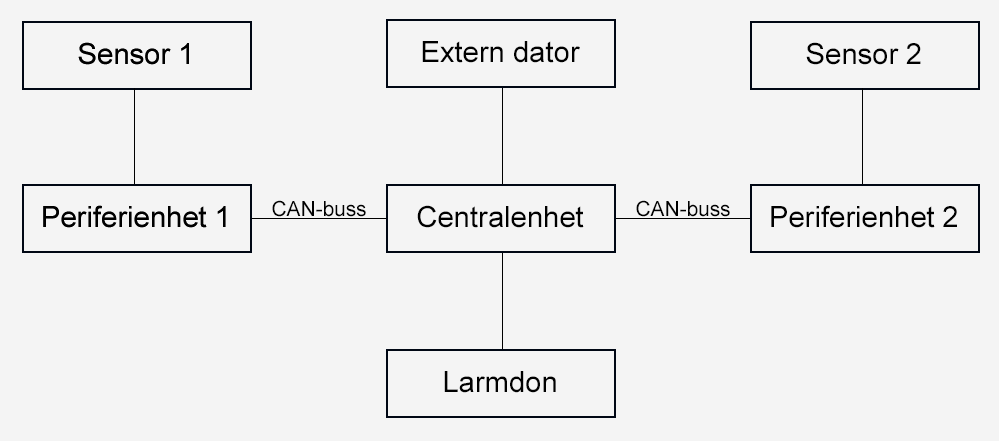
\includegraphics[width=\textwidth]{blockschema.png}
    \caption{Preliminärt blocksschema över larmsystemet}
    %\label{fig:my_label}
\end{figure}

Centralenheten kommunicerar med periferienheterna genom en \textit{Controller Area Network}-buss. Periferienheterna undersöker ändringar hos deras sensorer och vid funnen ändring rapporteras detta till centralenheten för larm. Inrapporteringen sker via ett meddelande på bussen som skapar ett avbrott hos centralenheten och aktiverar larmdonet.
% Ändringar hos sensorer undersöks av periferi...

Centralenheten måste kunna identifiera vilken periferienhet som skickat meddelandet och förstå varför det skickades. Identifikationen sker via kommunikation med en extern dator för att ge användaren en tydlig bild om var larmet uppstod.

\section{Resursplan}

E-mailadresser och ansvarsområden finns angivna i följade lista. Ansvar syftar på att den ansvarige ska se till att arbetet blir gjort, men inte att den ansvarige är skyldig att göra allt.

\subsection{Gruppmedlemmar och ansvarsområden}

\begin{description}
    \item[Titus Blosse, administrativt dokumentansvarig:] Ansvarar för att mötesprotokoll förs och att de olika rapporterna som ska skrivas under projektets gång såväl påbörjas som skickas in i tid.

    E-mail: titus.blosse@gmail.com

    \item[Viktor Frideen, planeringsansvarig:] Ansvarar för att informera gruppen om hur arbete med projektet och dess delmål fortgår och även för att uppmärksamma gruppen om de hamnar efter planeringen.

    E-mail: viktor.frideen@outlook.com

    \item[Nazif Kadiroglu, teknik dokumentansvarig:] Ansvarar för att all kod i projektet är dokumenterad.

    E-mail: nazif.kadiroglu1@gmail.com

    \item[Markus Moen, testansvarig:] Ansvarar för att tester på både hårdvara och mjukvara testas och dokumenteras.

    E-mail: markus.offersten@gmail.com

    \item[Lukas Schiavone, kodansvarig:] Ansvarar för att gruppen följer den kodstandard de har satt.

    E-mail: luksch1121@gmail.com

    \item[Fredrik Österström, gruppledare och resursansvarig:] Ansvarar för att kommunikation med kursens lärare, gruppmöten, hårdvarans tillgänglighet och att de verktyg gruppen har valt för kommunikation och versionhantering används.

    E-mail: fredrik.osterstrom@hotmail.com
\end{description}

\subsection{Hård- och mjukvara}

Hårdvaran för detta projekt finns tillgänglig i rum 4209 i EDIT-huset på Chalmers campus. Detta rum och hårdvaran bokas via doodle. Länkar till bokningssystemet finns tillgängliga på kurshemsidan. Hårdvaran som finns tillgänglig är:

\begin{itemize}
    \item 3x MD407 kort
    \item 1x Avståndsmätare (ultraljud), HC-SR04
    \item 1x Vibrationssensor, "Flying-Fish" SW-18010P
    \item 1x Keypad
    \item 1x 7-segmentsdisplay
    \item 2x 4-polig RJ-11 kabel (används för CAN-bussen)
    \item 1x RJ-11 förgrening
    \item 2x Tiopolig flatkabel
    \item 3x USB-kabel
    \item 1x Kopplingsplatta
\end{itemize}

Programspråket C kommer användas för att skriva mjukvaran. Den IDE (Integrated Design Environment) som kommer användas är CodeLite. då de kan simulera MD407-korten. Detta är fördelaktigt eftersom gruppmedlemmarna redan har erfarenthet med denna IDE. GitHub används för versionshantering.

En del av arbetet kan ske på distans, icke desto mindre test på hårdvaran kräver att gruppmedlemmar är på plats i Chalmers. Kommunikationen för arbete på distans är via Discord, som stödjer både röst- och textbaserad kommunikation samt skärm- och videodelning.

\section{Milstolpar}


\begin{table}[H]
    \centering
        \begin{tabular}{ |c|c|c| }\hline
            Nr & Beskrivning & Datum \\\hline\hline
            %\multirow{3}{4em}{Multiple row} & cell2 & cell3 \\
            1 & Projektplan klar & 11/09-20 \\\hline
            2 & Dörrlarm klart & 18/09-20 \\\hline
            3 & Rörelselarm klart & 25/09-20 \\\hline
            4 & Centralenhet delvis avklarad & 02/10-20 \\\hline
            5 & Första utkast slutrapport & 02/10-20 \\\hline
            6 & Centralenhet och periferienheter sammankopplade & 09/10-20 \\\hline
            7 & Opposition avklarad & 09/10-20 \\\hline
            8 & Andra utkast slutrapport & 16/10-20 \\\hline
            9 & Slutrapport avklarad & 30/10-20 \\\hline
        \end{tabular}
        % Text underneath the table
        \caption{Milstolpar för projektet}
        % Label for reference usage
        \label{table:milstolpar}
\end{table}

För att underlätta projektet har arbetet delats in i nio olika milstolpar. Dessa milstolpar är placerade på fredagen innan kursens officiella deadlines, då det lämnar utrymme för mer arbete efter milstolparna om så behövs. 

Programmeringsarbetet har delats in i fyra delar. Först utvecklas dörrlarmet och sedan rörelselarmet. Därefter utvecklas centralenheten och slutligen skall periferienheterna och centralenheten sammankopplas. 

\section{Aktiviteter}

Gruppmedlemmarna förväntas spendera 200h vardera med ett totalt antal mantimmar motsvarande 1200h. Tiden som varje medlem i gruppen förväntas lägga ner innefattar all tid som spenderas under projektets gång.

\begin{table}[H]
    \begin{center}
        \begin{tabular}{ |c|c|c| }\hline
            Nr & Beskrivning & Tidsåtgång \\\hline\hline
            1 & Föreläsningar (8 st på 2h, ett skrivseminarium på 3h, 6 personer) & 114h \\\hline
            2 & Dokumentationsläsning & 50h \\\hline
            3 & Framtagning av LaTeX-mallar & 18h \\\hline
            4 & Projektmöten (2h/vecka, 9 veckor, 6 personer) & 108h \\\hline
            5 & Skrivande av protokoll, kallelser etc & 20h \\\hline
            6 & Arbeta med projektplan & 120h \\\hline
            7 & Rapportutkast & 120h \\\hline
            8 & Renskrivande av Rapportutkast 1 & 15h \\\hline
            9 & Rapportutkast 2 & 80h\\\hline
            10 & Renskrivning av rapportutkast 2 & 10h \\\hline
            11 & Oppositionsrapport & 40h\\\hline
            12 & Slutföring av projektrapport & 110h\\\hline
            13 & Programmering av periferienhet, dörr & 40h \\\hline
            14 & Programmering av periferienhet, rörelse & 40h \\\hline
            15 & Programmering av centralenhet & 60h \\\hline
            16 & Tester och testrapport & 100h\\\hline
            17 & Granskning av kod & 60h \\\hline
            18 & Teknisk dokumentation & 60h \\\hline
            19 & Förbered/genomför demonstration & 35h \\\hline
        \end{tabular}
        \caption{Aktivitetslista för projektet}
        \label{table:aktivitetslista}
    \end{center}
\end{table}

Projektet har delats upp i aktiviteter för att gruppen ska ha koll på vad som ska genomföras under projektets gång. Noterbart är att aktiviteterna har givits en uppskattad tidsåtgång i tabell \ref{table:aktivitetslista}. Tidsåtgången kan variera under projektets gång och kan avvika från den upskattade tidsåtgången. Tabell \ref{table:aktivitetslista} ovan visar att gruppen sammanlagt kommer lägga cirka 1200 timmar på projektet. Dessa timmar sorteras in på 19 aktiviteter och 4 kategorier.

%Första kategorin, som innefattar nummer 1-4, berör det administrativa. Andra kategorin, det vill säga nummer 5-12, berör rapport delen av projektet. Denna del kommer tillmestadels handla om att skriva om projektet, renskrivning och oppositionsrapport. Tredje kategorin, där nummer 13-19 ingår, kommer att handla om det praktiska arbetet. Här berörs allt från programmering av periferienheter till tester och demonstrationer.

\begin{description}
    \item[Första kategorin] innefattar aktivitet 1-3 och berör inläsningen och förarbetet gruppen kommer göra under arbetets gång. (182h)
    
    \item[Andra kategorin] innefattar aktivitet 4-5 och berör det administrativa arbetet. (128h)
    
    \item[Tredje kategorin] innefattar aktivitet 6-12 och berör den skriftliga delen av projektet. (495h)
    
    \item[Fjärde kategorin] innefattar aktivitet 13-19 berör den praktiska delen av projektet. Här berörs programmering, test och demonstrationer. (395h)
    
    \end{description}

% !dessa timmar, !denna del, !här

\section{Tidsplan}
\begin{figure}[H]
    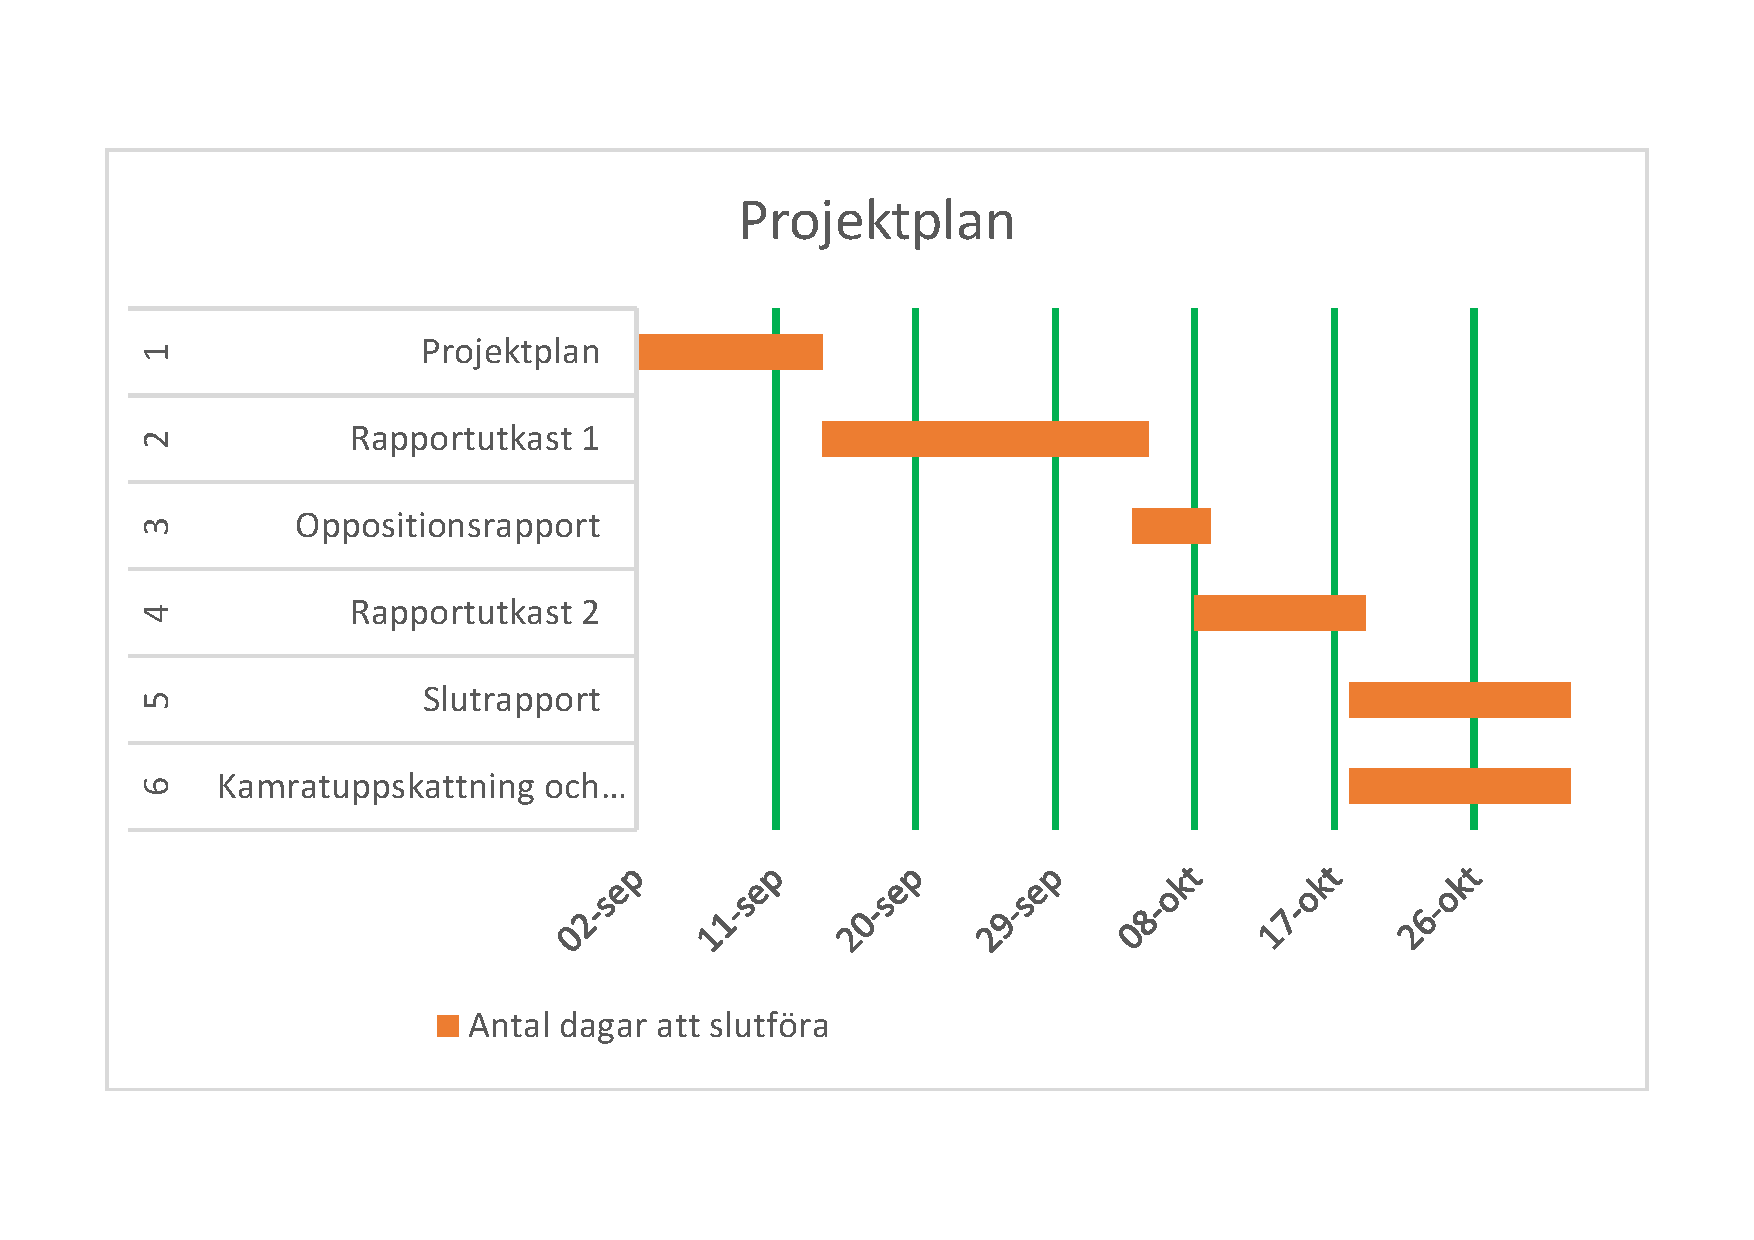
\includegraphics[width=\textwidth]{Gantschema.pdf}
    \caption{Gantt-schema}
    \label{figure:gantt}
\end{figure}

Aktiviteter som inte visas i \ref{figure:gantt} sker kontinuerligt under projektets gång. De olika aktiviteterna och deras tidåtgång har lagts upp i ett gantt-schema. De första två veckorna är lågintensiva där gruppen får en överbklick på hur projektet skall se ut och även arbeta på projektplaneringen. Efter dessa veckor blir det högintensivt där gruppen sätter igång med det praktiska och även arbetar på projektrapporten. Utöver detta ska även opositionsrapporten skrivas. Sista 2 veckorna går åt till att färdigställa rapporten och förbereda inför demonstration. Det redovisade gantt-schemat ger gruppen en överblick på ungefär när deadlinen på de olika rapporterna är samt hur många dagar gruppen har på sig på de angivna aktiviteterna.

\section{Mötesplan}

Mötestillfällen där alla gruppmedlemmar inklusive mentor medverkar.

\begin{table}[H]
    \begin{center}
        \begin{tabular}{ |c|c|c| }\hline
            Datum & tid & Lokal \\\hline\hline
            02/09-20 & 13:00-15:00 & ED4209 \\\hline
            09/09-20 & 15:00-17:00 & Zoom \\\hline
            16/09-20 & 13:00-15:00 & Zoom \\\hline
            23/09-20 & 13:00-15:00 & Zoom \\\hline
            30/09-20 & 13:00-15:00 & Zoom \\\hline
            07/10-20 & 13:00-15:00 & Zoom \\\hline
            14/10-20 & 13:00-15:00 & Zoom \\\hline
            21/10-20 & 13:00-15:00 & Zoom \\\hline
            28/10-20 & 13:00-15:00 & Zoom \\\hline
        \end{tabular}
        \caption{Tabell över mötestillfällen}
        \label{table:motesplan}
    \end{center}
\end{table}

\section{Kommunikationsplan}

\begin{table}[H]
    \centering
    \begin{tabular}{ |c|c|c|c| }\hline
     Vad & När & Till & Hur \\\hline
     Dagsordning LV1 & 02/09-20 & Alla & Anslag i canvas \\\hline
     Mötesprotokoll LV1 & 02/09-20 & Alla & Anslag i canvas \\\hline
     Dagsordning LV2 & 09/09-20 & Alla & Anslag i canvas \\\hline
     Mötesprotokoll LV2 & 10/09-20 & Alla & Anslag i canvas \\\hline
     Projektplan & 09/13-20 & Lärarteam & Canvas inlämning \\\hline 
     Dagsordning LV3 & 16/09-20 & Alla & Anslag i canvas \\\hline
     Mötesprotokoll LV3 & 17/09-20 & Alla & Anslag i canvas \\\hline
     Dagsordning LV4 & 23/09-20 & Alla & Anslag i canvas \\\hline
     Mötesprotokoll LV4 & 24/09-20 & Alla & Anslag i canvas \\\hline
     Dagsordning LV5 & 30/09-20 & Alla & Anslag i canvas \\\hline
     Mötesprotokoll LV5 & 01/10-20 & Alla & Anslag i canvas \\\hline
     Projektrapport utkast 1 & 04/10-20 & Lärarteam & Canvas inlämning \\\hline
     Dagsordning LV6 & 07/10-20 & Alla & Anslag i canvas \\\hline
     Mötesprotokoll LV6 & 08/10-20 & Alla & Anslag i canvas \\\hline
     Dagsordning LV7 & 14/10-20 & Alla & Anslag i canvas \\\hline
     Mötesprotokoll LV7 & 15/10-20 & Alla & Anslag i canvas \\\hline
     Projektrapport utkast 2 & 18/10-20 & Läratteam & Canvas inlämning \\\hline
     Dagsordning LV8 & 21/10-20 & Alla & Anslag i canvas \\\hline
     Mötesprotokoll LV8 & 22/10-20 & Alla & Anslag i canvas \\\hline
     Dagsordning LV9 & 28/10-20 & Alla & Anslag i canvas \\\hline
     Mötesprotokoll LV9 & 29/10-20 & Alla & Anslag i canvas \\\hline
     Projektrapport & 03/11-20 & Lärarteam & Canvas inlämning \\\hline
    \end{tabular}
    \caption{Kommunikationsplan för projektet}
    \label{table:kommunikationsplan}
\end{table}

För intern kommunikation används både Discord och Messenger. Gruppmöten med handledare kommer i första hand att ske igenom Zoom.

\section{Kvalitetsplan}

För att verifiera att systemet och dess delsystem fungerar behöver tester utföras. Tester av mjukvaran kan i viss mån göras i simulator, men innan den kan markeras som klar måste den testas i hårdvaran. Vid test av de olika komponenterna skall följande mall fyllas i:

\begin{description}
\item[Komponent] Den del av systemet ska testas.

\item[Testsyfte] Vilken funktionalitet som testas.

\item[Utförande] Hur testet ska utföras och vilka specifika fall som testas.

\item[Resultat] Resultatet av testet.

\item[Analys] Vad testresultatet innebär; om komponenten fungerar som planerat, behöver testas ytterligare eller om vidare utveckling krävs.
\end{description}

%\section{Spelregler}

% Tells the compiler what reference system to use
\bibliographystyle{IEEEtran}
% Prints the reference list at the end of the file
\bibliography{referenser.bib}

\end{document}
